\chapter{การทดสอบและการวิจารณ์}
\label{ch:results}
วิธีการตรวจสอบแสตมป์ตามที่นำเสนอในบทที่ 3 ได้รับการทวนสอบ (verification) ด้วยการทดลองกับภาพแสตมป์จริงและแสตมป์ปลอมอย่างละ 20 ภาพ ในหัวข้อ 4.1 จะบอกถึงข้อมูลของกล้องและระบบคอมพิวเตอร์รวมทั้งโปรแกรมที่ใช้ในการทดสอบ หัวข้อ 4.2 จะบอกถึงผลที่ได้จากการทดสอบ และหัวข้อ 4.3 เป็นการวิจารณ์ผลการทดสอบที่ได้


\section{การเตรียมการในการทดสอบ}
 \subsection{ระบบฮาร์ดแวร์และซอฟท์แวร์ที่ใช้ในการทดสอบ} 
 \label{sec:setup}
ในการทดลองเพื่อทดสอบวิธีการที่นำเสนอ ระบบการถ่ายภาพแสตมป์แบบง่าย ตามที่นำเสนอในบทที่ 3 ได้ถูกสร้างขึ้น เพื่อการถ่ายภาพแสตมป์ที่ใช้ในการทดสอบ สำหรับกล้องที่ใช้ในการถ่ายภาพเป็นกล้องดิจิทัลซึ่งมีข้อมูลของกล้องตามที่แสดงในตารางที่~\ref{tab:camera}

\begin{table}[htb]
\caption{ข้อมูลกล้องที่ใช้ในการถ่ายภาพสแตมป์}
\label{tab:camera}
\begin{tabular}{ll}
\hline
รุ่นของกล้อง            &NIKON D5200\\
จำนวนจุดพิกเซล      &24.1 megapixels\\
เลนส์                    &18 -55 VR\\
ระยะโฟกัส             &Contrast Detect (sensor\\
ความเร็วชัตเตอร์      &30 sec-1/4000 sec\\
การซูม                  &35-55 mm\\
\hline
\end{tabular}
\end{table} 


วิธีการที่นำเสนอได้ถูกนำสร้างบนแพล็ตฟอร์ม Matlab โดยการเขียนเป็นโปรแกรมรันบนคอมพิวเตอร์ส่วนบุคคล

\subsection{ข้อมูลสำหรับการทดลอง}
ภาพของแสตมป์สำหรับการทดสอบได้จากการถ่ายภาพด้วยกล้องถ่ายภาพตามหัวข้อ~\ref{sec:setup} ในการทดสอบระบบจำเป็นต้องมีภาพแสตปม์ทั้งที่เป็นแสตมป์จริง และแสตมป์ปลอมจำนวน 2 เซต โดยทั้งหมดเป็นสแตมป์ที่ได้จากสรรพากรเขตพื้นที่จังหวัดอุบลราชธานี โดยมีรายละเอียดของแสตมป์ตัวอย่างตามตารางที่~\ref{tab:data}

\begin{table}[htb]
\caption{ข้อมูลแสตมป์ที่ใช้ในการทดลอง}
\label{tab:data}
\begin{tabular}{ll}
\hline 
ชนิดของแสตมป์       &เป็นแสตมป์สุราของสรรพากรเขตพื้นที่จังหวัดอุบลราชธานี\\
จำนวนแสตมป์ทั้งหมด          &50 แสตมป์\\
จำนวนแสตมป์จริง               & 25 แสตมป์\\
จำนวนแสตมป์ปลอม            &25 แสตมป์\\
\hline
\end{tabular}
\end{table} 

\subsection{การเรียนรู้เพื่อหาเส้นตรงที่ใช้เป็นเกณฑ์การตรวจสอบ}

ตามวิธีการที่นำเสนอในบทที่ 3 การตรวจสอบว่าแสตมป์เป็นของจริงหรือของปลอม จะต้องมีการเรียนรู้เพื่อสร้างเกณฑ์สำหรับการตรวจสอบ ซึ่งเป็นเส้นตรงบนระนาบ $w-h$ โดย 
               $w$ เป็นความกว้างของฮิสโตแกรมของภาพระดับสีเขียวของตรานกวายุภักษ์ในแสตมป์ และ
               $h$ เป็นความสูงที่สุดของอิสโตแกรมของภาพระดับสีเขียวของตรานกวายุภักษ์ในแสตมป์ 
              กระบวนการในการเรียนรู้เป็นไปตามที่อธิบายไว้ในหัวข้อ~\ref{sec:training}

สำหรับในการทดสอบนี้ ได้เลือกภาพแสตมป์จำนวน 10 ภาพเป็นสแสตมป์จริงและแสตมป์ปลอมอย่างไร 5 ภาพ เพื่อใช้เป็นเซตของภาพสำหรับการเรียนรู้ (training set) ผลการเรียนรู้เป็นไปตามที่แสดงในรูปที่~\ref{fig:training-result} ซึ่งเป็นสมการเส้นตรงตามสมการที่~\ref{eq:classification-line}

\begin{figure}[!ht]
\centering
\vspace{2em}
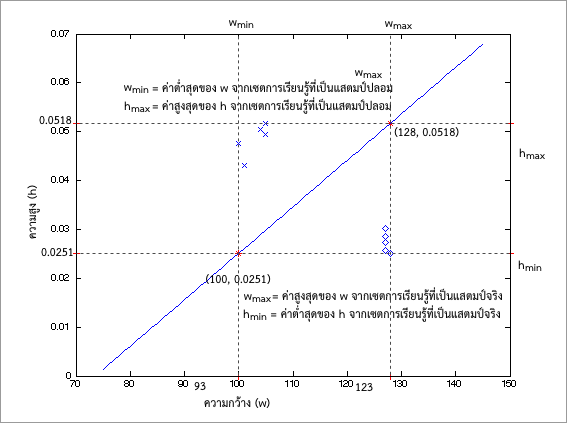
\includegraphics[width=0.9\textwidth]{training-result-n5}
\vspace{2em}
\caption{กราฟจากการพล็อตจุดพิกัด $(w,h)$ ที่ได้จากการเรียนรู้ด้วยเซตของภาพสำหรับการเรียนรู้}
\label{fig:training-result}
\end{figure}

\begin{eqnarray}
%\frac{h - h_{min}}{w - w_{min}} &=& \frac{h_{max} - h_{min}}{w_{max}-w_{min}} \nonumber\\
h &=& m*(w - w_{0}) + h_{0} \label{eq:classification-line}\\
m &=& \frac{h_{max} - h_{min}}{w_{max}-w_{min}} = 8.881\times 10^{-4}\nonumber\\
w_0 &=& w_{min} = 100\nonumber\\
h_0 &=& h_{min}  = 0.0251\nonumber\\\nonumber
\end{eqnarray}

 โดยที่  
 \begin{itemize}
 \item $w_{min}$ เป็นค่าต่ำสุดของ $w$ ที่ได้จากชุดข้อมูลสำหรับการเรียนรู้ กลุ่มแสตมป์ปลอม  
 \item[]จากการทดลองได้ $w_{min} = 100$
 \item $w_{max}$ เป็นค่าสูงสุดของ $w$ ที่ได้จากชุดข้อมูลสำหรับการเรียนรู้ กลุ่มแสตมป์จริง 

 \item[]จากการทดลองได้ $w_{max} = 128$
\item $h_{min}$ เป็นค่าต่ำสุดของ $h$ ที่ได้จากชุดข้อมูลสำหรับการเรียนรู้ กลุ่มแสตมป์จริง 

\item[]จากการทดลองได้ $h_{min} = 0.0251$ 
\item $h_{max}$ เป็นค่าสูงสุดของ $h$ ที่ได้จากชุดข้อมูลสำหรับการเรียนรู้ กลุ่มแสตมป์ปลอม 

\item[]จากการทดลองได้ $h_{max} = 0.0518$ 
\item $m$ เป็นความชันของเส้นแบ่ง จากการทดลองได้
\item $(w_0, h_0)$ เป็นจุด ๆ หนึ่งบนเส้นแบ่งในที่นี้เลือกใช้จุด $(w_{min}, h_{min})$
 \end{itemize}
 

           

\section{ผลการทดสอบและการวิจารณ์}
วิธีการที่นำเสนอมี 2 ขั้นตอนหลัก คือ (1) การตัดเอาเฉพาะตรานกวายุภักษ์ และ (2) การตรวจสอบว่านกวายุภักษณ์ที่ตัดมาเป็นของจริงหรือของปลอม ดังนั้นในการทดสอบจึงแบ่ง 2 ขั้นตอน 
โดยภาพที่ที่ใช้ในการทดสอบเป็นภาพที่ไม่อยู่ในเซตของการเรียนรู้ โดยเป็นภาพแสตมป์จริง 20 ภาพ และภาพแสตมป์ปลอม  20  ภาพ

\subsection{ผลการตัดรูปนกวายุภักษ์} 
 ในขั้นตอนแรกเป็นการทดสอบเพื่อพิจารณาผลการตัดเอาเฉพาะตรานกวายุภักษ์ รูปที่~\ref{fig:bird-cut-result-r}~และ~\ref{fig:bird-cut-result} แสดงผลการตัดสำหรับแสตมป์ที่เป็นแสตมป์จริง และแสตมป์ปลอมตามลำดับ

\begin{figure}[!ht]
\centering
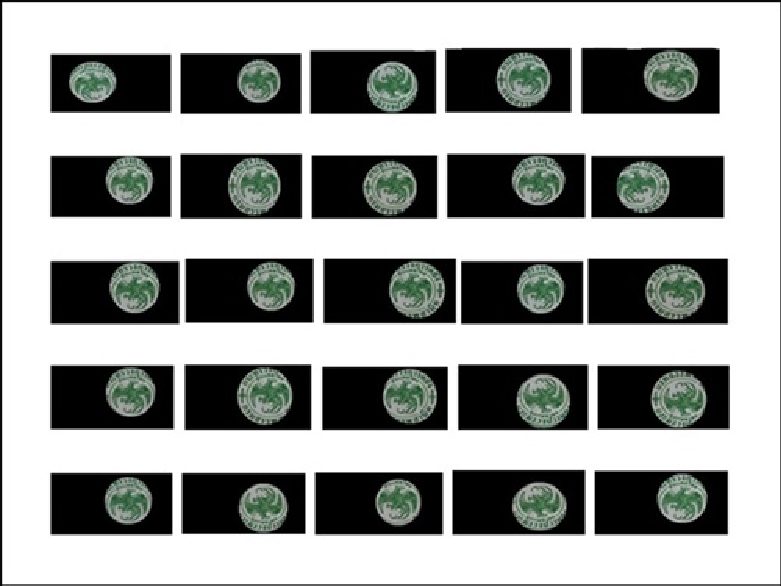
\includegraphics[width=0.9\textwidth]{bird-cut-result-r}
\caption{ภาพนกวายุภักษ์ที่ได้จากผลการตัดจากภาพแสตมป์จริงที่ใช้ในการทดสอบ}
\label{fig:bird-cut-result-r}
\end{figure}

\begin{figure}[!ht]
\centering
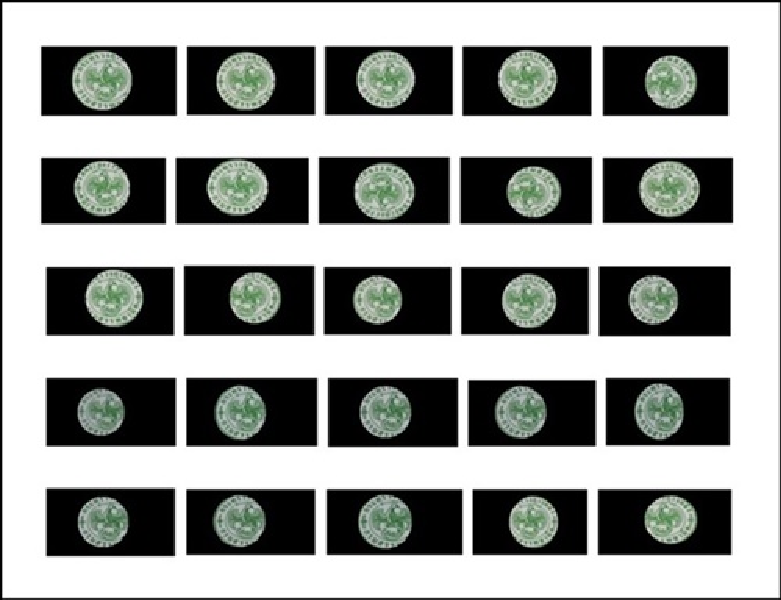
\includegraphics[width=0.9\textwidth]{bird-cut-result-f}
\caption{ภาพนกวายุภักษ์ที่ได้จากผลการตัดจากภาพแสตมป์ปลอมที่ใช้ในการทดสอบ}
\label{fig:bird-cut-result-f}
\end{figure}
 

จากรูปที่~\ref{fig:bird-cut-result-r}~และ~\ref{fig:bird-cut-result-f} การตัดเอาภาพของนกวายุภักษ์เพื่อไปใช้ในการตรวจสอบนั้น ไม่ได้ถูกต้องทั้งหมด ภาพการตัดที่ไม่ถูกต้องจะมีลักษณะที่มีบางส่วนภายในกรอบของรูปครุฑที่หายไป และอาจจะมีบางภาพที่มีส่วนอื่นเพิ่มขึ้นมา  ทั้งนี้เพราะตรานกวายุภักษ์ซี่งอยู่ในกรอบวงกลม ภายในภาพแสตมป์ที่ใช้ทดลอบนั้น ตัววงกลมล้อมรอบรูปครุฑจะไม่สมดุล  กล่าวคือจะมีลักษณะเป็นวงรี  ทำให้การตัดซึ่งเป็นการตัดด้วยวงกลมมีความคลาดเคลื่อนในบางส่วน เหตุผลที่ภาพเป็นวงรีนั้นมาจากขั้นตอนการถ่ายภาพ ซึ่งควบคุมให้ภาพเป็นวงกลมทั้งหมดได้ยาก

อย่างไรก็ตามผลการตัดที่คลาดเคลื่อนดังกล่าวนี้มีผลกระทบกับการแยกแยะไม่มาก เพราะลักษณะเด่นที่ใช้ในการวิเคราะเป็นคุณสมบัติของการกระจายของสีเขียวของส่วนที่เป็นตรานกวายุภักษ์ ซึ่งผลของการคลาดเคลื่อนจะเป็นผลต่อจุดพิกัดของ $(w, h)$ อยู่บ้างแต่มีไม่มากพอที่จะให้เกิดการย้ายกลุ่ม

\begin{figure}[!hb]
\centering
\vspace{2em}
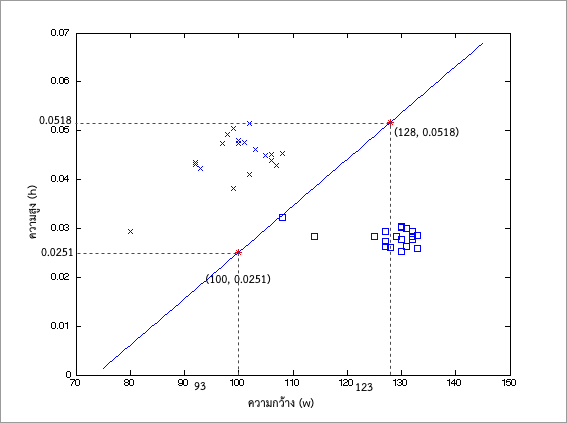
\includegraphics[width=0.9\textwidth]{testing-result}
\vspace{2em}
\caption{กราฟจากการพล็อตจุดพิกัด $(w,h)$ ที่หาได้จากภาพตรานกวายุภักษ์ที่ตัดมาจากภาพแสตมป์ที่ใช้ทดสอบ}
\label{fig:classification-result}
\end{figure}

\subsection{ผลการแยกแยะชนิดของแสตมป์} 

ภาพที่ได้จากการตัดรูปนกวายุภักษ์จะถูกนำไปตรวจสอบว่าเป็นภาพของแสตมป์จริงหรือของแสตมป์ปลอม โดยการนำข้อมูลสีเขียวของภาพที่ตัดได้ไปหาฮิสโตแกรม แล้วปรับให้ฮิสโตแกรมไปทำให้อยู่ในช่วงเดียวกันคือมีค่าระหว่าง 0 ถึง 1 เหมือนกัน ทั้งนี้เพราะภาพที่ตัดมาอาจมีขนาดภาพไม่เท่ากัน จากนั้นจึงหาค่า $w$ และ $h$ ของแต่ละภาพ นำค่า $w$ และ $h$ ที่ได้ไปเปรียบกับเส้นแบ่งที่ได้จากการเรียนรู้ ถ้าจุด $(w,h)$ อยู่เหนือเส้นแบ่งแสดงว่าเป็นภาพตรานกวายุภักษ์นั้นเป็นของแสตมป์ปลอม รูปที่~\ref{fig:classification-result} แสดงผลพล็อตจุด $(w,h)$ ของภาพทดสอบทั้งหมด โดยกากบาทเป็นจุดของภาพทดสอบที่เป็นแสตมป์ปลอม ส่วนเครื่องหมายรูปเพชรเป็นจุดของภาพทดสอบที่เป็นแสตมป์จริง 



ถ้าจุดเครื่องหมายกากบาทอยู่ใต้เส้นแบ่ง แสดงว่าเป็นการตัดสินผิดจากของปลอมเป็นของจริง ซึ่งไม่พบกรณีนี้เกิดขึ้นจากภาพตัวอย่างที่ใช้ทดสอบ
ถ้าจุดรูปเพชร อยู่เหนือเส้นแบ่ง แสดงว่าเป็นการตัดสินผิดจากของจริงเป็นของปลอม ซึ่งไม่พบกรณีนี้เกิดจากภาพตัวอย่างที่ใช้ทดสอบ
สรุปได้ว่าวิธีที่นำเสนอสามารถตรวจสอบแสตมป์ตัวอย่างจำนวน 40 แสตมป์ได้ทั้งหมด



จากผลการทดสอบพบว่าวิธีที่นำเสนอสามารถตรวจสอบแสตมป์ตัวอย่างที่ใช้ทดสอบทั้งหมด 40 แสตมป์ได้ทั้งหมด ซึ่งแสดงว่าวิธีที่นำเสนอมีโอกาสที่จะถูกนำไปใช้งานได้จริง อย่างไรก็ตามแม้ยังมีประเด็นที่ต้องให้ความสนใจดังต่อไปนี้
\begin{enumerate}
\item ตามวิธีที่นำเสนอนั้น การตัดรูปครุฑมีความสำคัญอย่างยิ่งเพราะเกณฑ์ในการตัดขึ้นอยู่กับฮิสโตแกรมของรูปครุฑเท่านั้น ถ้าตัดรูปครุฑผิดฮิสโตแกรมอาจจะมีคุณสมบัติที่แตกต่าง ทำให้ตัดสินผิด หรือในบางกรณีตัดสินใจไม่ได้เลย   แต่อย่างไรก็ตามแม้ว่าภาพที่ถ่ายมาวงกลมจะปรากฏเป็นวงรี ผลการตัดก็ยังถูกต้องในแง่ที่สามารถตัดเอาส่วนใหญ่ของรูปครุฑออกมาได้ทุกกรณีของภาพตัวอย่าง 
\item ปัญหาที่อาจจะเกิดได้กับการตัดตรานกวายุภักษ์คือ กรณีที่แสตมป์ที่ติดอยู่ที่ขวดมีความไม่สมบูรณ์ เช่น มีบางส่วนหายไป หรือแสตมป์มีการขาด ซึ่งจะเป็นปัญหาวิจัยในอนาคตเพื่อทำให้สามารถนำวิธีการที่นำเสนอไปใช้งานได้จริง
\item สำหรับขั้นตอนการหาจุดพิกัด (w, h) จากอิสโตแกรมของรูปครุฑ มีความเป็นไปได้ที่อาจจะเกิดปัญหาขึ้นเมื่อในการนำวิธีที่นำเสนอไปใช้งานจริง ในกรณีที่มีความไม่เท่ากันของแสงที่ใช้ ซึ่งอาจจะส่งผลต่อเส้นแบ่งที่ได้จากการเรียนรู้มาก่อน จึงเป็นอีกกรณีหนึ่งที่จะต้องทำการศึกษาเพื่อเพิ่มเติม
\item ประเด็นสุดท้ายคือวิธีการที่นำเสนอตั้งอยู่บนฐานของแสตมป์ปลอมเพียงกลุ่มเดียว ดังนั้นจึงเป็นไปไม่ได้ที่จะบอกว่าวิธีการที่นำเสนอนี้สามารถตรวจสอบแสตมป์ได้ทุกชนิด 
\end{enumerate}



 
 







          
           

